\apendice{Documentación de usuario}

\section{Introducción}
Esta memoria presenta la documentación completa de usuario para ReservApp, un sistema integral de gestión de reservas desarrollado con tecnología Java Spring Boot. ReservApp está diseñado para facilitar la administración y reserva de establecimientos, proporcionando una plataforma intuitiva tanto para usuarios finales como para administradores del sistema.

El sistema permite a los usuarios realizar reservas en establecimientos asignados, gestionar convocatorias de reuniones y administrar sus perfiles personales. Los administradores pueden gestionar usuarios, establecimientos, perfiles del sistema y supervisar todas las reservas realizadas.

Esta documentación está estructurada para guiar al usuario paso a paso a través de todas las funcionalidades disponibles, desde el registro inicial hasta las operaciones más avanzadas de administración del sistema.

\section{Requisitos de usuarios}
El acceso a la aplicación está condicionado únicamente a la disponibilidad de una conexión a internet, dado su diseño como plataforma web. Esto garantiza una total compatibilidad multiplataforma, permitiendo su uso desde dispositivos móviles, tabletas y ordenadores. No obstante, para optimizar la experiencia de usuario, se aconseja el acceso desde un ordenador.

\section{Instalación}
Dado que se trata de una aplicación web, no es necesaria ninguna instalación local. Se puede acceder a la aplicación de forma inmediata a través del enlace \url{https://reservapp-1u8c.onrender.com/}.

\newpage

\section{Manual del usuario}
A continuación se detallan las operaciones que se pueden realizar en la aplicación.

\subsection{Acceso a la Aplicación}

\begin{figure}[H]
	\centering
		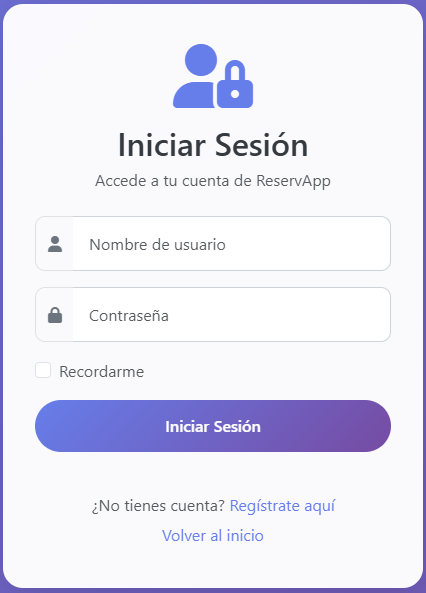
\includegraphics[width=0.5\linewidth]{reservapp_login}
	\caption{Página inicial de la aplicación.}
	\label{fig:reservapp_login}
\end{figure}

\subsubsection{Registro de un nuevo usuario}
Nada más acceder a la aplicación, se mostrará por defecto la página de inicio, tal y como se puede ver en la figura ~\ref{fig:reservapp_login}. Si es la primera vez que se utiliza la aplicación, será necesario crear una cuenta para poder acceder a las funcionalidades de reserva. Estos son los pasos a seguir:

\begin{enumerate}
   \item \textbf{Acceder a la página de registro}:

   \begin{itemize}
      \item Desde la página de inicio, hacer clic en ``Regístrate aquí''.
      \item O navegar directamente a ``/registro''.
   \end{itemize}
   \item \textbf{Completar el formulario de registro}:
   \begin{itemize}

      \begin{figure}[H]
         \centering
         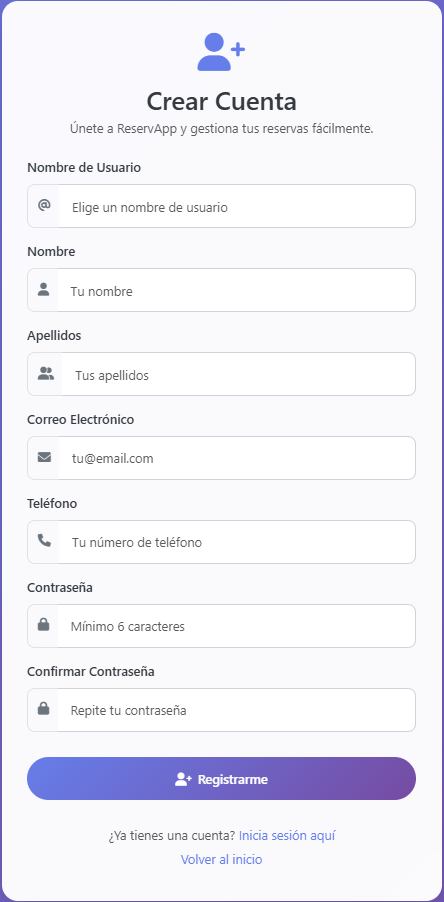
\includegraphics[width=0.5\linewidth]{reservapp_registro}
         \caption{Página para el registro de usuario.}
         \label{fig:reservapp_registro}
      \end{figure}

      \item Al acceder, se mostrará una página como se muestra en la figura ~\ref{fig:reservapp_registro}.
      \item \textbf{ID de Usuario}: Introducir un identificador único de 3-10 caracteres alfanuméricos (sin espacios ni símbolos especiales).
      \item \textbf{Nombre}: Introducir el nombre (máximo 50 caracteres).
      \item \textbf{Apellidos}: Introducir los apellidos (máximo 50 caracteres).
      \item \textbf{Correo Electrónico}: Introducir una dirección de email válida y única.
      \item \textbf{Contraseña}: Crear una contraseña segura.
      \item \textbf{Confirmar Contraseña}: Repetir la contraseña para verificación.
      \item \textbf{Teléfono}: Introducir número de teléfono (5-12 caracteres).
   \end{itemize}
   \item \textbf{Enviar el formulario}:
   \begin{itemize}
      \item Hacer clic en ``Registrarse''.
      \item El sistema validará los datos y creará la cuenta.
      \item Se mostrará un mensaje de confirmación.
   \end{itemize}
\end{enumerate}

\textbf{Notas importantes}:
\begin{itemize}
   \item El ID de usuario y el correo electrónico deben ser únicos en el sistema.
   \item Todos los campos son obligatorios.
   \item El sistema encripta automáticamente las contraseñas.
\end{itemize}

\subsubsection{Inicio de sesión (login)}
En caso de tener un usuario previamente creado, se podrá acceder a la aplicación con las credenciales existentes. Estos son los pasos a seguir:

\begin{enumerate}
   \item \textbf{Acceder a la página de login}:

   \begin{itemize}
      \item Navegar a /login o hacer clic en ``Iniciar Sesión''.
   \end{itemize}
   \item \textbf{Introducir credenciales}:
   \begin{itemize}
      \item \textbf{Usuario}: Introducir el ID de usuario registrado.
      \item \textbf{Contraseña}: Introducir la contraseña correspondiente.
      \item Opcionalmente, marcar ``Recordarme'' para mantener la sesión activa.
   \end{itemize}
   \item \textbf{Iniciar sesión}:
   \begin{itemize}
      \item Hacer clic en ``Iniciar Sesión''.
      \item El sistema redirigirá al menú principal tras la autenticación exitosa.
   \end{itemize}
\end{enumerate}

\textbf{Mensajes de error comunes}:
\begin{itemize}
   \item ``Usuario o contraseña incorrectos'': Verificar las credenciales introducidas.
   \item Usuario bloqueado: Contactar con el administrador del sistema.
\end{itemize}

\subsubsection{Cierre de Sesión}
Cerrar la sesión actual de forma segura. Estos son los pasos a seguir:

\begin{enumerate}
   \item Desde cualquier página del sistema, hacer clic en el botón ``Cerrar Sesión'' en la barra de navegación.
   \item El sistema cerrará la sesión y redirigirá a la página de login.
\end{enumerate}

\subsection{Navegación Principal}

\subsubsection{Menú Principal}
El menú principal es el centro de control del sistema, organizado en secciones según el rol del usuario.

\begin{figure}[H]
	\centering
		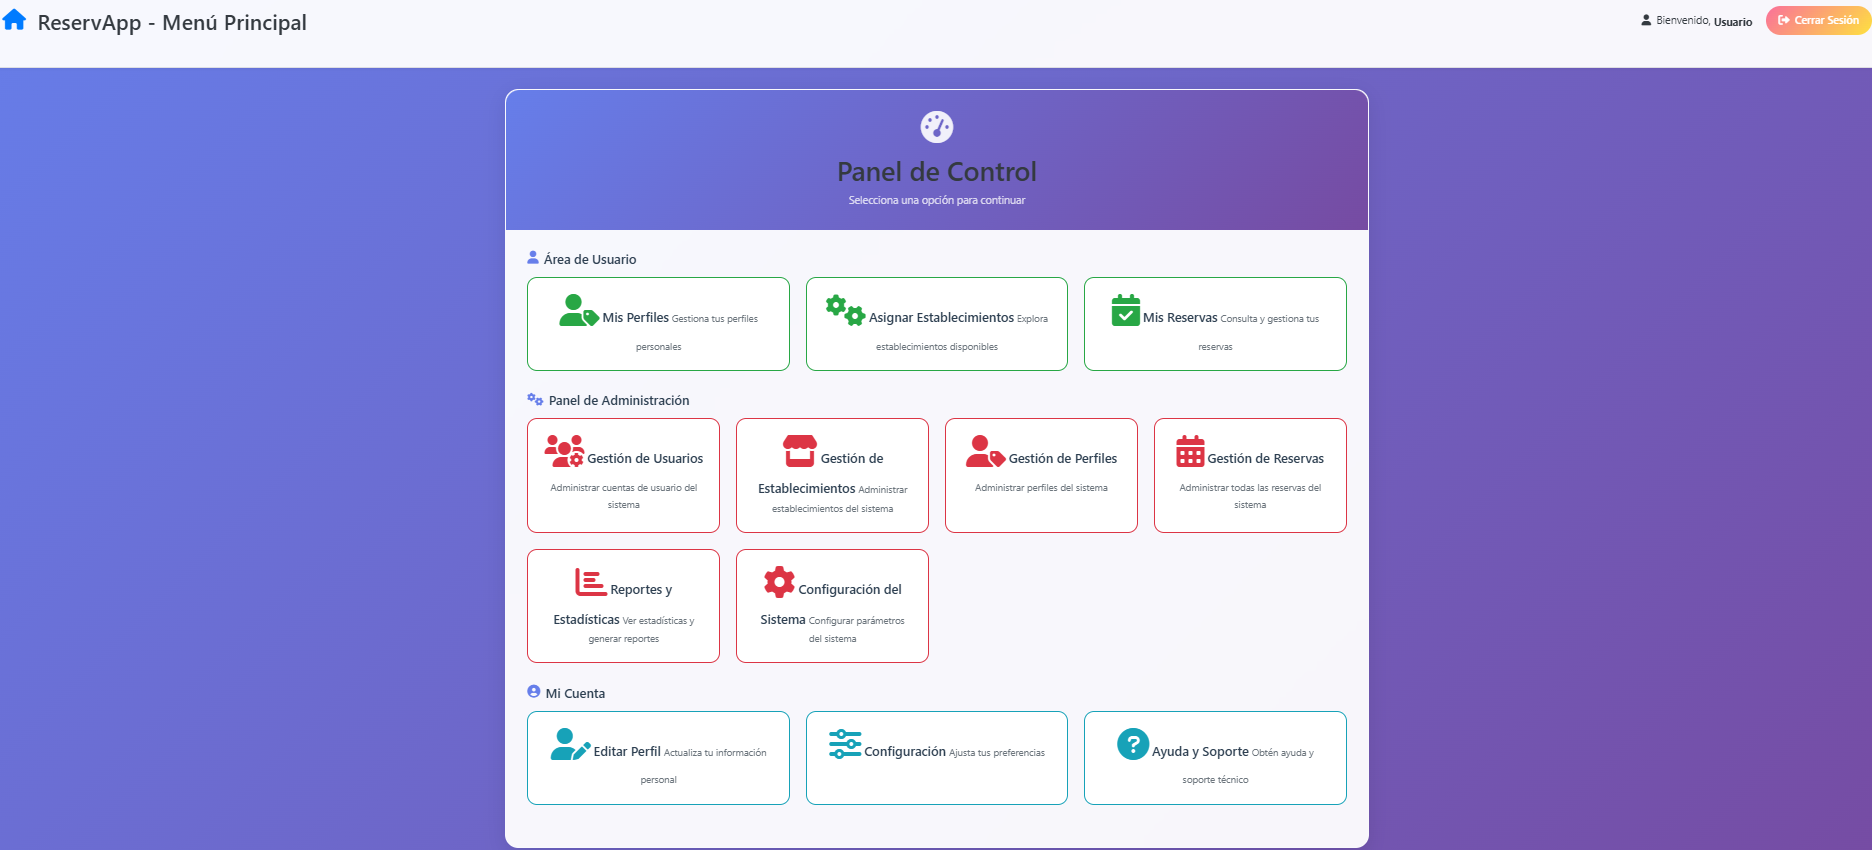
\includegraphics[width=0.9\linewidth]{reservapp_menu_principal_admin}
	\caption{Menú Principal para usuario administrador.}
	\label{fig:reservapp_menu_principal_admin}
\end{figure}

\begin{figure}[H]
	\centering
		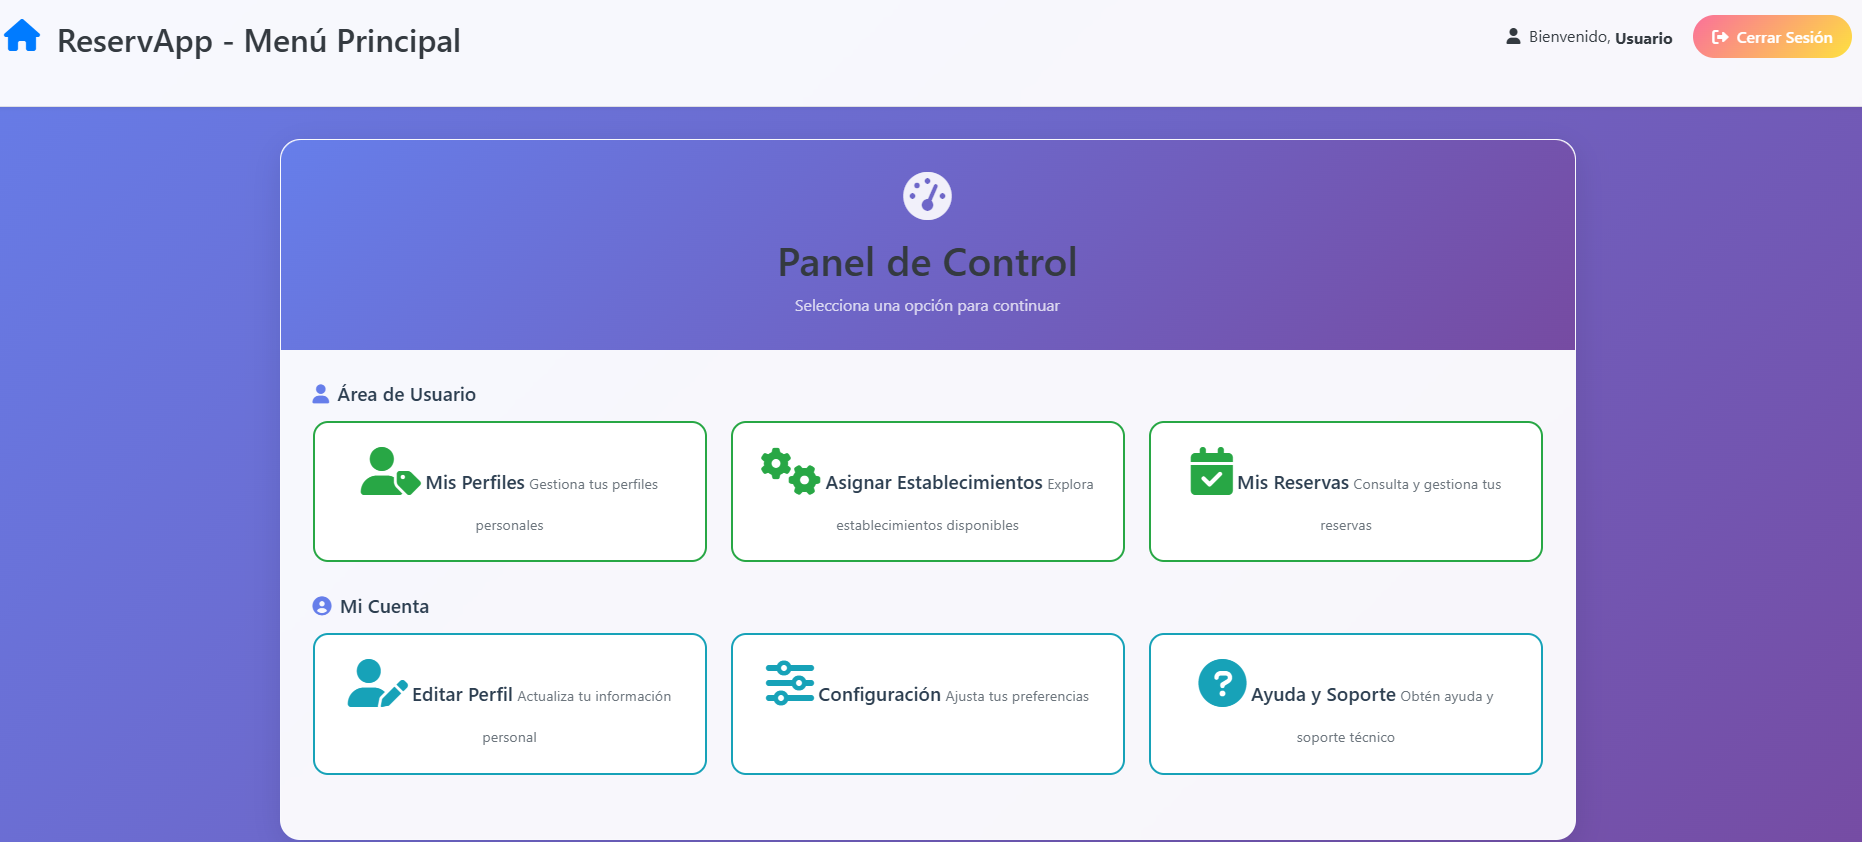
\includegraphics[width=0.9\linewidth]{reservapp_menu_principal_no_admin}
	\caption{Menú Principal para usuario no administrador.}
	\label{fig:reservapp_menu_principal_no_admin}
\end{figure}

\begin{itemize}
   \item Para todos los usuarios, tal y como se muestra en la figura~\ref{fig:reservapp_menu_principal_no_admin}, aparecen disponibles las siguientes secciones:
   \begin{itemize}
      \item \textbf{Área de Usuario}:
      \begin{itemize}
         \item Mis Perfiles: Gestión de perfiles personales.
         \item Asignar Establecimientos: Explorar y solicitar acceso a establecimientos
         \item Mis Reservas: Consultar y gestionar reservas personales
      \end{itemize}
      \item \textbf{Mi Cuenta}:
      \begin{itemize}
         \item Editar Perfil: Actualizar información personal.
         \item Configuración: Ajustar preferencias del usuario.
         \item Ayuda y Soporte: Acceder a documentación y soporte.
      \end{itemize}
   \end{itemize}
   \item Para todos los administradores, tal y como se muestra en la figura~\ref{fig:reservapp_menu_principal_admin}, además de las opciones que se muestra para el esto de usuarios, aparecen disponibles las siguientes secciones:
   \begin{itemize}
      \item \textbf{Panel de Administración}:
      \begin{itemize}
         \item Gestión de Usuarios: Administrar cuentas de usuario.
         \item Gestión de Establecimientos: Administrar establecimientos del sistema.
         \item Gestión de Perfiles: Administrar perfiles del sistema.
         \item Gestión de Reservas: Supervisar todas las reservas.
         \item Reportes y Estadísticas: Ver estadísticas del sistema.
         \item Configuración del Sistema: Configurar parámetros globales.
      \end{itemize}
   \end{itemize}
\end{itemize}

\subsection{Gestión de Resrervas}

\subsubsection{Visualizar Mis Reservas}
Permite consultar los establecimientos disponibles para realizar reservas, tal y como se ilustra en la figura~\ref{fig:reservapp_mis_reservas}. Estos son los pasos a seguir:

\begin{figure}[H]
	\centering
		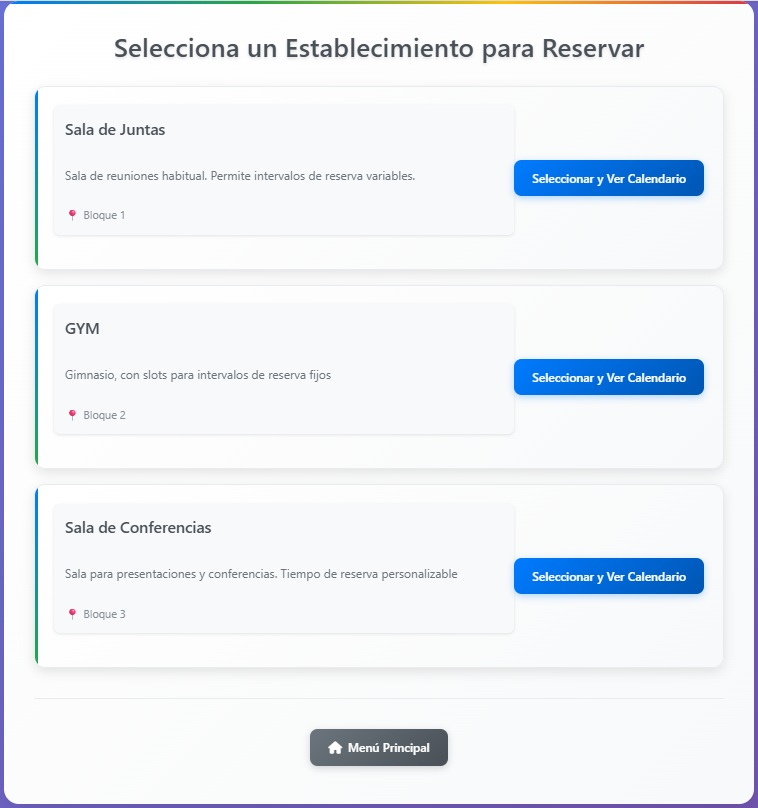
\includegraphics[width=0.5\linewidth]{reservapp_mis_reservas}
	\caption{Página de ``Mis Reservas''.}
	\label{fig:reservapp_mis_reservas}
\end{figure}

\begin{enumerate}
   \item \textbf{Acceder a ``Mis Reservas''}:
   \begin{itemize}
      \item Desde el menú principal, hacer clic en ``Mis Reservas''.
      \item O navegar directamente a /misreservas.
   \end{itemize}
   \item \textbf{Seleccionar establecimiento}:
   \begin{itemize}
      \item Se mostrará una lista de establecimientos asignados al usuario.
      \item Cada establecimiento muestra:
      \begin{itemize}
         \item Nombre del establecimiento.
         \item Descripción.
         \item Dirección.
      \end{itemize}
      \item Hacer clic en ``Seleccionar y Ver Calendario'' para el establecimiento deseado.
   \end{itemize}
\end{enumerate}

\subsubsection{Crear Nueva Reserva}
Permite crear una nueva reserva para un establecimiento en concreto, tal y como se ilustra en la figura~\ref{fig:reservapp_mis_reservas}. Estos son los pasos a seguir:

\begin{figure}[H]
	\centering
		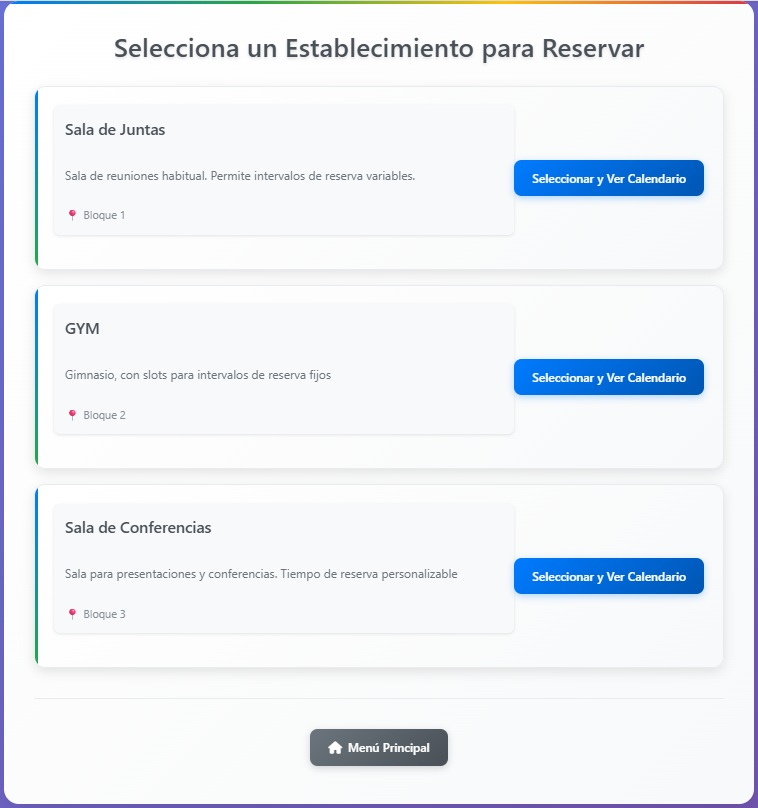
\includegraphics[width=0.5\linewidth]{reservapp_mis_reservas}
	\caption{Página de ``Mis Reservas'' donde se muestran los establecimientos asignados.}
	\label{fig:reservapp_mis_reservas}
\end{figure}

\begin{enumerate}
   \item \textbf{Acceder al calendario de reservas}:
   \begin{itemize}
      \item Desde ``Mis Reservas'', seleccionar un establecimiento.
      \item Se mostrará el calendario de reservas del establecimiento.
   \end{itemize}
   \item \textbf{Revisar información del establecimiento}:
   \begin{itemize}
      \item \textbf{Detalles}: Dirección, teléfono, estado.
      \item \textbf{Aforo}: Número máximo de personas por horario (si aplica).
      \item \textbf{Horarios de apertura}: Días y horas disponibles para reservas.
   \end{itemize}
   \item \textbf{Seleccionar fecha y hora}:
   \begin{itemize}
      \item \textbf{Fecha}: Seleccionar una fecha futura en el calendario.
      \item \textbf{Horario}: Dependiendo del establecimiento:
      \begin{itemize}
         \item \textbf{Slots predefinidos}: Seleccionar de una lista de horarios disponibles.
         \item \textbf{Horario libre}: Introducir hora de inicio y fin manualmente.
      \end{itemize}
   \end{itemize}
   \item \textbf{Configurar convocatoria (opcional)}:
   \begin{itemize}
      \item \textbf{Enlace de reunión}: Introducir URL de videoconferencia (Google Meet, Zoom, Teams, etc.).
      \item \textbf{Observaciones}: Añadir notas, agenda o temas a tratar.
      \item \textbf{Invitar usuarios}:
      \begin{itemize}
         \item Buscar usuarios por nombre, apellido, ID o email.
         \item Seleccionar usuarios de los resultados de búsqueda.
         \item Los usuarios seleccionados aparecerán en la lista de invitados.
      \end{itemize}
   \end{itemize}
   \item \textbf{Confirmar reserva}:
   \begin{itemize}
      \item Revisar todos los datos introducidos.
      \item Hacer clic en ``Confirmar Reserva''.
      \item El sistema validará la disponibilidad y creará la reserva.
      \item El sistema validará la disponibilidad y creará la reserva.
   \end{itemize}
\end{enumerate}

\textbf{Validaciones del sistema}:
\begin{itemize}
   \item La fecha debe ser futura.
   \item El horario debe estar dentro de las franjas de apertura del establecimiento.
   \item No debe exceder el aforo máximo del establecimiento.
   \item La hora de fin debe ser posterior a la hora de inicio
\end{itemize}
